% =====================================================================
%  ECONSCHOOL — PROBLEMS SHEET
%  One solved problem (with a TikZ figure) + one near-twin exercise.
%
%  Compile:  pdflatex hybrid-preferences.tex   (run twice for the footer)
%  No font installation needed: text and maths are Computer Modern
%  (Latin Modern where available), the same maths face the site renders
%  with KaTeX.
% =====================================================================
\documentclass[11pt]{article}

% ---- Fonts ----------------------------------------------------------
% Latin Modern if available (it is on MacTeX); base Computer Modern
% otherwise. Either way the maths face is Computer Modern.
\IfFileExists{lmodern.sty}{\usepackage[T1]{fontenc}\usepackage{lmodern}}{}

% ---- Core packages --------------------------------------------------
\usepackage{amsmath,amssymb}
\usepackage[a4paper,top=2.3cm,bottom=2.4cm,left=2.6cm,right=2.6cm]{geometry}
\usepackage{graphicx}
\usepackage{xcolor}
\usepackage{microtype}
\usepackage{enumitem}

% ---- Figures --------------------------------------------------------
\usepackage{tikz}
\usepackage{pgfplots}
\pgfplotsset{compat=1.18}
\usetikzlibrary{arrows.meta}

% ---- Layout ---------------------------------------------------------
\setlist[enumerate]{leftmargin=1.6em,itemsep=0.35em,topsep=0.3em}
\setlist[itemize]{leftmargin=1.6em,itemsep=0.2em,topsep=0.2em}
\setlength{\parindent}{0pt}
\setlength{\parskip}{0.6em}
\linespread{1.05}

% ---- Brand palette (mirrors src/styles/global.css) ------------------
\definecolor{bg}{HTML}{FAF7F2}             % cream background
\definecolor{ink}{HTML}{2A2620}            % body text
\definecolor{inksoft}{HTML}{4A4239}        % secondary text
\definecolor{inkfaint}{HTML}{7A6F62}       % tertiary / italics
\definecolor{violet}{HTML}{5A1BA6}         % titles
\definecolor{violetsoft}{HTML}{7A4FC4}     % sub-headings
\definecolor{terracotta}{HTML}{A03A2C}     % accents, links, budget line
\definecolor{terracottasoft}{HTML}{C66B5B} % light fills
\definecolor{sage}{HTML}{8AA08A}           % dividers, guide ray
\definecolor{sagesoft}{HTML}{C8D2C0}       % footer rule
\definecolor{rule}{HTML}{E5DDD0}           % hairline rules

% ---- Figure styles --------------------------------------------------
% A small reusable set for the diagrams these sheets need. Add curve
% colours per topic (demand/supply, cost curves, ...) as required.
\pgfplotsset{
  microecon/.style={
    width=8.4cm, height=6.4cm,
    axis lines=middle,
    axis line style={-{Stealth[length=2mm]}, ink},
    tick label style={font=\footnotesize, color=inksoft},
    label style={font=\small, color=inksoft},
    every axis x label/.style={at={(ticklabel* cs:1.02)}, anchor=west},
    every axis y label/.style={at={(ticklabel* cs:1.02)}, anchor=south},
    xmin=0, ymin=0,
    tick align=outside,
    enlargelimits=false,
  },
}
\tikzset{
  indiff/.style={ink, thick},                             % indifference curve (optimal)
  indiffsoft/.style={ink, thin},                          % indifference curve (context)
  budget/.style={terracotta, thick},                      % budget line
  optimum/.style={circle, fill=violet, inner sep=1.6pt},  % optimal bundle
  optset/.style={violet, line width=1.7pt},               % set of optimal bundles
}

% ---- Document colour ------------------------------------------------
\color{ink}
\pagecolor{bg}        % cream page; comment out this line for white

% ---- Links ----------------------------------------------------------
\usepackage[hidelinks]{hyperref}
\hypersetup{colorlinks=true, urlcolor=terracotta, linkcolor=terracotta}

% ---- Small reusable pieces ------------------------------------------
\newcommand{\eyebrow}[1]{{\color{terracotta}\textls[110]{\scshape #1}}}
% ES mark: the logo if present, a typographic fallback otherwise.
\newcommand{\esmark}{%
  \IfFileExists{es-logo.png}
    {\raisebox{-0.34\height}{
\includegraphics[height=5mm]{es-logo.png}}}
    {{\color{violet}\fontsize{20}{20}\selectfont\scshape ES}}}
\newcommand{\sagerule}{\par\vspace{0.25em}{\color{sage}\rule{\linewidth}{0.6pt}}\par\vspace{0.15em}}
\newcommand{\heading}[1]{\par\vspace{1.1em}{\color{violet}\large\bfseries #1}\par\vspace{0.25em}}
\newcommand{\subheading}[1]{\par\vspace{0.7em}{\color{violetsoft}\bfseries #1}\par\vspace{0.1em}}
\newcommand{\MU}{\mathrm{MU}}   % upright marginal-utility symbol

% ---- Footer ---------------------------------------------------------
\usepackage{fancyhdr}
\pagestyle{fancy}
\fancyhf{}
\renewcommand{\headrulewidth}{0pt}
\renewcommand{\footrulewidth}{0.4pt}
\renewcommand{\footrule}{{\color{sagesoft}%
  \vskip-\footruleskip\vskip-\footrulewidth
  \hrule height\footrulewidth width\headwidth}}
\fancyfoot[L]{\color{inkfaint}\footnotesize econschool.in}
\fancyfoot[C]{\color{inkfaint}\footnotesize\thepage}
\fancyfoot[R]{\color{inkfaint}\footnotesize youtube.com/@econ.school}

% =====================================================================
\begin{document}

% ---------- Masthead -------------------------------------------------
\noindent
\begin{tabular*}{\linewidth}{@{}l@{\extracolsep{\fill}}r@{}}
  \eyebrow{To go with the lectures} & \esmark
\end{tabular*}
\sagerule

% ---------- Title (replace per sheet) --------------------------------
{\color{violet}\fontsize{26}{30}\selectfont Hybrid preferences\par}
\vspace{0.2em}
{\color{inkfaint}\itshape Consumer theory \;\textperiodcentered\; Problem~4
 \quad\textperiodcentered\quad
 Video: \href{https://youtu.be/DYMhGCBVAOE}{youtu.be/DYMhGCBVAOE}\par}
\sagerule

% =====================================================================
\heading{Solved problem}

A student buys bread and butter. A slice of bread is worth something on its own; a pat of butter is worth something only spread on a slice --- one pat per slice --- and a buttered slice is worth twice a plain one. Butter with no bread does nothing. Writing
\begin{itemize}
  \item $x$: pats of butter, at price $p_x$;
  \item $y$: slices of bread, at price $p_y$,
\end{itemize}

tastes are $u(x,y)=\min\{x+y,\,2y\}$, a hybrid of substitutes and complements. For every $(p_x,p_y,M)$, determine the demand correspondence $(X^d,Y^d)(p_x,p_y,M)$.

\subheading{Solution}
The student solves
\[
  \begin{aligned}
    \max_{(x,y)\in\mathbb{R}^2_+}\quad & \min\{x+y,\,2y\}\\
    \text{s.t.}\quad & p_x x + p_y y \le M.
  \end{aligned}
\]

First read the utility. Since $x+y\le 2y$ exactly when $x\le y$,
\[
  u(x,y)=\min\{x+y,\,2y\}=y+\min\{x,y\}=
  \begin{cases}
    x+y & x\le y,\\[2pt]
    2y  & x\ge y.
  \end{cases}
\]
So a pat of butter only helps while some slice is still plain ($x<y$); once every slice is buttered ($x\ge y$) extra butter is wasted. The student would never pay for wasted butter, so the optimum has $x\le y$, where $u=x+y$ and butter and bread are perfect substitutes at rate $1:1$. It remains to maximise $x+y$ on the budget subject to $x\le y$, which turns on the cost per unit of utility, $p_x$ for butter against $p_y$ for bread.

If $p_x>p_y$, bread is the cheaper source of utility --- a buttered slice costs $p_x+p_y$ for $2$ units, beaten by two plain slices at $2p_y$ --- so the student buys only bread, $(0,M/p_y)$. If $p_x<p_y$, butter is cheaper and the student wants all of it, but butter past $x=y$ is wasted, so the choice is pinned to the kink $x=y$, giving $\bigl(\tfrac{M}{p_x+p_y},\tfrac{M}{p_x+p_y}\bigr)$. If $p_x=p_y$, then $x+y=M/p_y$ at every bundle on the budget with $x\le y$, so all of them are optimal at once. Collecting these,
\[
  (X^d,Y^d)(p_x,p_y,M)=
  \begin{cases}
    \bigl\{(0,\,M/p_y)\bigr\} & p_x>p_y,\\[4pt]
    \bigl\{(x,y)\in\mathbb{R}^2_+ : p_x x+p_y y=M,\ y\ge x\bigr\} & p_x=p_y,\\[4pt]
    \Bigl\{\bigl(\tfrac{M}{p_x+p_y},\,\tfrac{M}{p_x+p_y}\bigr)\Bigr\} & p_x<p_y.
  \end{cases}
\]

Notice that when $p_x=p_y$, the utility-maximization problem has multiple solutions, so demand here is a correspondence, or set-valued function.


\begin{center}
% ---- (a) p_x > p_y : bread corner ----------------------------------
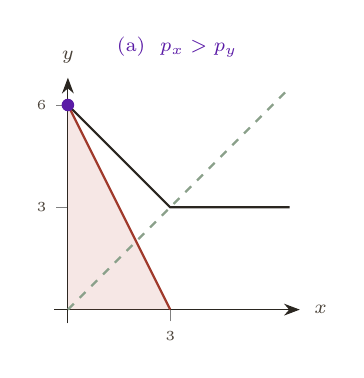
\begin{tikzpicture}
  \begin{axis}[microecon, width=4.7cm, height=4.7cm,
      xmin=-0.4, xmax=6.8, ymin=-0.4, ymax=6.8,
      xlabel={$x$}, ylabel={$y$}, xtick={3}, ytick={3, 6},
      tick label style={font=\tiny, color=inksoft},
      label style={font=\scriptsize, color=inksoft},
      title style={font=\scriptsize, color=violet, yshift=-2pt},
      title={(a)\ \ $p_x>p_y$}, clip mode=individual]
    \addplot[draw=none, fill=terracottasoft, fill opacity=0.16]
      coordinates {(0,0) (3,0) (0,6)} \closedcycle;                 % budget set
    \draw[sage, thick, dashed] (axis cs:0,0) -- (axis cs:6.5,6.5);  % x=y
    \draw[indiff] (axis cs:0,6) -- (axis cs:3,3) -- (axis cs:6.5,3);% u=6 curve
    \addplot[budget, domain=0:3] {6 - 2*x};                         % 2x+y=6
    \node[optimum] at (axis cs:0,6) {};                             % optimum (0,6)
  \end{axis}
\end{tikzpicture}
\hfill
% ---- (b) p_x = p_y : whole segment ---------------------------------
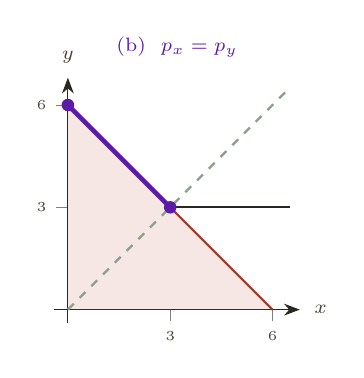
\begin{tikzpicture}
  \begin{axis}[microecon, width=4.7cm, height=4.7cm,
      xmin=-0.4, xmax=6.8, ymin=-0.4, ymax=6.8,
      xlabel={$x$}, ylabel={$y$}, xtick={3,6}, ytick={3,6},
      tick label style={font=\tiny, color=inksoft},
      label style={font=\scriptsize, color=inksoft},
      title style={font=\scriptsize, color=violet, yshift=-2pt},
      title={(b)\ \ $p_x=p_y$}, clip mode=individual]
    \addplot[draw=none, fill=terracottasoft, fill opacity=0.16]
      coordinates {(0,0) (6,0) (0,6)} \closedcycle;
    \draw[sage, thick, dashed] (axis cs:0,0) -- (axis cs:6.5,6.5);
    \draw[indiff] (axis cs:3,3) -- (axis cs:6.5,3);                 % flat arm of u=6
    \addplot[budget, domain=0:6] {6 - x};                           % x+y=6
    \draw[optset] (axis cs:0,6) -- (axis cs:3,3);                   % optimal segment
    \node[optimum] at (axis cs:0,6) {};
    \node[optimum] at (axis cs:3,3) {};
  \end{axis}
\end{tikzpicture}
\hfill
% ---- (c) p_x < p_y : the kink --------------------------------------
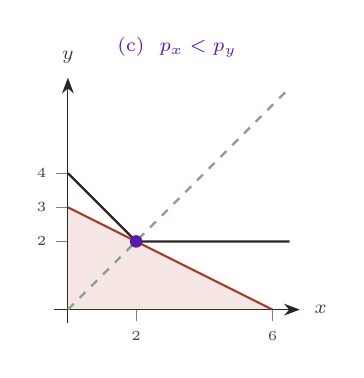
\begin{tikzpicture}
  \begin{axis}[microecon, width=4.7cm, height=4.7cm,
      xmin=-0.4, xmax=6.8, ymin=-0.4, ymax=6.8,
      xlabel={$x$}, ylabel={$y$}, xtick={2,6}, ytick={2,3,4},
      tick label style={font=\tiny, color=inksoft},
      label style={font=\scriptsize, color=inksoft},
      title style={font=\scriptsize, color=violet, yshift=-2pt},
      title={(c)\ \ $p_x<p_y$}, clip mode=individual]
    \addplot[draw=none, fill=terracottasoft, fill opacity=0.16]
      coordinates {(0,0) (6,0) (0,3)} \closedcycle;
    \draw[sage, thick, dashed] (axis cs:0,0) -- (axis cs:6.5,6.5);
    \draw[indiff] (axis cs:0,4) -- (axis cs:2,2) -- (axis cs:6.5,2);% u=4 curve
    \addplot[budget, domain=0:6] {3 - 0.5*x};                       % x+2y=6
    \node[optimum] at (axis cs:2,2) {};                             % kink optimum
  \end{axis}
\end{tikzpicture}
\end{center}
\vspace{-0.1em}
{\color{inkfaint}\footnotesize\itshape
 Figure~1.\enspace The three price cases, all at $M=6$ on common axes. The
 dashed line is $x=y$, where the indifference curves kink; the violet mark is
 the optimum. \textbf{(a)} $p_x>p_y$ ($p_x=2$, $p_y=1$): the budget is steeper
 than the slope-$1$ arm, so it reaches the highest indifference curve only at the bread corner
 $(0,6)$. \textbf{(b)} $p_x=p_y$ ($=1$): the slope-$1$ arm lies along the budget, so every
 bundle from $(0,6)$ to the kink $(3,3)$ is optimal --- the violet segment.
 \textbf{(c)} $p_x<p_y$ ($p_x=1$, $p_y=2$): the budget is flatter than the sloped arm but steeper than the flat arm, so it supports the kink $(2,2)$.\par}
\sagerule

% =====================================================================
\heading{Exercise}

A student buys rice and beans. Each is filling on its own, and a serving of each eaten together makes a balanced plate that is worth an extra unit. Writing
\begin{itemize}
  \item $x$: servings of rice, at price $p_x$;
  \item $y$: servings of beans, at price $p_y$,
\end{itemize}

tastes are
\[
  u(x,y)=\min\{2x+y,\,x+2y\}=(x+y)+\min\{x,y\}.
\]

\begin{enumerate}
  \item For every $(p_x,p_y,M)$, find the demand correspondence $(X^d,Y^d)(p_x,p_y,M)$. \emph{Hint:} $u=2x+y$ when $x\le y$ and $u=x+2y$ when $x\ge y$, with the kink on $x=y$; in each region compare the utility per dollar of the two goods.

  \item Show that demand is set-valued at two price ratios, not one. Identify them and describe the optimal set at each.

  \item Take $p_x=3$, $p_y=2$, $M=12$, and find the optimal bundle. Then take $p_x=4$, $p_y=2$ with $M=12$ and describe the optimal set.
\end{enumerate}

\subheading{Extension: one threshold or two}

\begin{enumerate}
  \setcounter{enumi}{3}
  \item In the solved problem demand was set-valued at a single price ratio, $p_x=p_y$; here it is set-valued at two. Explain the difference from the slopes of the two indifference-curve arms in each problem.
\end{enumerate}

\medskip
{\color{inksoft}\emph{Checking your work.}\enspace To discuss the exercise, join
 the community forum at \href{https://econschool.in}{econschool.in}.\par}

\end{document}
